\documentclass[conference]{IEEEtran}

\usepackage[T1]{fontenc}
\usepackage[utf8]{inputenc}
\usepackage{cite}
\usepackage{amsmath,amssymb}
\usepackage{graphicx}
\usepackage{booktabs}
\usepackage{hyperref}
\usepackage{url}
\usepackage{array}
\usepackage{balance}

\hypersetup{colorlinks=true,linkcolor=black,citecolor=black,urlcolor=black}

\begin{document}

\title{Explainable Machine Learning for Retail Sales Prediction:\\A Comparative Study on the Rossmann Store Sales Dataset}

\author{
    \IEEEauthorblockN{Aman Ismail Mullick}
    \IEEEauthorblockA{
        Faculty of Computer Science and Automation\\
        Technische Universit\"{a}t Ilmenau, Ilmenau, Germany\\
        aman-ismail.mullick@tu-ilmenau.de
    }
}

\maketitle

\begin{abstract}
Retail sales prediction is a central operational challenge, yet high-performing machine learning models rarely explain what drives a given prediction. This paper compares Linear Regression, Random Forest, and XGBoost on the Rossmann Store Sales dataset — 1,017,209 daily sales records from 1,115 German drugstores (2013--2015) — and applies TreeSHAP to both ensemble models for post-hoc explainability. After preprocessing and feature engineering yielding 24 input features, models are evaluated on a held-out set of 168,868 samples. XGBoost achieved the best results: MAE~=~\euro854.15, RMSE~=~\euro1,198.13, $R^{2}$~=~0.8512, and MAPE~=~13.78\%, outperforming Linear Regression by 57.6\% and Random Forest by 17.4\% on MAE. TreeSHAP identified competition proximity (mean $|\text{SHAP}|$~=~0.193), promotional activity (0.182), and store identity (0.167) as the dominant sales drivers. Notably, short competition distance carries a \emph{positive} SHAP attribution — proxying commercial-zone density rather than a competitive penalty — a pattern not visible from importance ranking alone. A store-level waterfall explanation for Store~161 demonstrates that SHAP attributions are directly interpretable by non-technical users. All results are evaluated on an 80/20 random held-out split within the 2013--2015 period; the study measures in-sample generalisation, not temporal out-of-sample forecasting.
\end{abstract}

\begin{IEEEkeywords}
retail sales prediction, explainable AI, SHAP, XGBoost, Random Forest, Rossmann dataset
\end{IEEEkeywords}

% -------------------------------------------------------
\section{Introduction}
% -------------------------------------------------------

Managing inventory, staffing, and promotional spend across a large retail network requires reliable daily sales predictions at the individual store level~\cite{hyndman2021}. Classical time-series approaches such as ARIMA~\cite{box1994} are interpretable but designed for single univariate sequences and do not incorporate the categorical and continuous features that characterise retail store behaviour. Tree-based ensemble methods have become the standard for structured tabular data~\cite{grinsztajn2022}, and the Rossmann Store Sales Kaggle competition (2015) confirmed their dominance in this domain.

Despite their accuracy, ensemble models create a deployment problem: store managers cannot verify or act on predictions they cannot understand. A prediction of \euro8,800 is useful; one that explains a promotional uplift of \euro1,200 offset by a competitive penalty is operationally actionable. SHAP (SHapley Additive exPlanations)~\cite{lundberg2017}, and its TreeSHAP variant~\cite{lundberg2020}, addresses this by providing feature attributions with game-theoretic guarantees of consistency and local faithfulness to the model.

This paper trains and compares all three models on the Rossmann dataset, applies TreeSHAP to both ensemble models, and demonstrates that store-level SHAP explanations translate directly into retail management decisions. Section~\ref{sec:related} reviews related work; Section~\ref{sec:method} describes the methodology; Section~\ref{sec:results} presents results; Section~\ref{sec:conclusion} concludes.

% -------------------------------------------------------
\section{Related Work}
\label{sec:related}
% -------------------------------------------------------

ARIMA and Holt-Winters smoothing~\cite{box1994} are standard univariate benchmarks but degrade when targets depend on interacting features such as promotions, competitor proximity, and store format. Random Forest~\cite{breiman2001} captures non-linear interactions through bootstrap-aggregated trees; XGBoost~\cite{chen2016} extends this with residual boosting, achieving lower bias on high-dimensional tabular data. LightGBM~\cite{ke2017} and CatBoost~\cite{prokhorenkova2018} offer further speed and categorical improvements, while LSTMs~\cite{hochreiter1997} and the Temporal Fusion Transformer~\cite{lim2021} address multi-horizon settings. Grinsztajn et al.~\cite{grinsztajn2022} and Shwartz-Ziv and Armon~\cite{shwartz2022} both showed that tree-based models consistently outperform neural methods on fixed-length tabular data, motivating the focus here.

LIME~\cite{ribeiro2016} approximates local model behaviour with a linear surrogate but is unstable across runs due to sampling randomness. SHAP~\cite{lundberg2017} distributes predictions across features via Shapley values from cooperative game theory, guaranteeing that contributions sum exactly to the prediction minus the baseline. TreeSHAP~\cite{lundberg2020} computes exact Shapley values for tree ensembles in polynomial time. Ribeiro et al.~\cite{ribeiro2016} showed that local explanations measurably increase stakeholder trust, and Dzyabura and Hauser~\cite{dzyabura2019} demonstrated that interpretable demand models improve promotional decision-making.

% -------------------------------------------------------
\section{Methodology and Experimental Setup}
\label{sec:method}
% -------------------------------------------------------

\subsection{Dataset and Preprocessing}

The Rossmann Store Sales dataset contains 1,017,209 daily sales records from 1,115 German drugstores (January 2013 -- July 2015), joined with store metadata. Records with closed stores or zero sales were excluded, leaving 844,338 samples. An 80/20 \emph{random} split (seed~42) yielded 675,470 training and 168,868 held-out samples. This split evaluates in-sample generalisation across the 2013--2015 period; it does not constitute a true out-of-sample temporal forecasting evaluation. A time-ordered split — training on 2013--2014 and testing on 2015 — would be required for that purpose and is identified as future work. The target variable has mean~\euro6,955.96, standard deviation~\euro3,103.82, and skewness~1.59.

Missing values were handled domain-specifically: \texttt{CompetitionDistance} (0.3\% missing) was replaced with the median (2,325~m); \texttt{CompetitionOpenSince} (31.8\% missing) and \texttt{Promo2} fields (49.9\% missing) were set to zero, encoding ``no recorded event.'' Twenty-four features were engineered: date decomposition (year, month, day, week, quarter), duration features (\texttt{CompetitionDuration} in months, \texttt{Promo2Duration} in weeks), binary retail-cycle flags (\texttt{IsWeekend}, \texttt{IsMonthStart}, \texttt{IsMonthEnd}), and label-encoded categoricals (\texttt{StoreType}, \texttt{Assortment}, \texttt{StateHoliday}, \texttt{PromoInterval}).

\subsection{Models and Evaluation}

Three models spanning increasing complexity were evaluated. \textbf{Linear Regression} is the interpretable baseline, assuming additive linear feature effects. \textbf{Random Forest}~\cite{breiman2001} trains 100 trees via bootstrap bagging (max depth~15, min leaf~5). \textbf{XGBoost}~\cite{chen2016} trains 500 trees sequentially (learning rate~0.05, max depth~6, L1~=~0.1, L2~=~1.0, subsample~0.80) with early stopping on validation RMSE. All models were evaluated using MAE, RMSE, $R^{2}$, and MAPE on the held-out set. TreeSHAP~\cite{lundberg2020} was applied to both ensemble models on 600 randomly sampled validation records, producing beeswarm plots, importance rankings, a dependence plot, and a waterfall explanation.

% -------------------------------------------------------
\section{Results and Discussion}
\label{sec:results}
% -------------------------------------------------------

\subsection{Model Performance}

Table~\ref{tab:performance} and Fig.~\ref{fig:comparison} summarise validation performance. Linear Regression's $R^{2}$~of 0.20 reflects its inability to model non-linear interactions between promotions, store type, and competition — the primary drivers of retail sales variance. Its MAPE of 33.66\% means predictions deviate by roughly one-third of actual sales. Random Forest raises $R^{2}$~to 0.77 by learning these interactions through deep trees. XGBoost achieves the best result on all four metrics, reducing MAE by 17.4\% over Random Forest and 57.6\% over Linear Regression; sequential boosting and L1/L2 regularisation jointly explain its advantage.

\begin{table}[t]
\centering
\caption{Validation Set Performance ($n = 168{,}868$)}
\label{tab:performance}
\setlength{\tabcolsep}{4pt}
\begin{tabular}{lcccc}
\toprule
\textbf{Model} & \textbf{MAE (\euro)} & \textbf{RMSE (\euro)} & $\boldsymbol{R^{2}}$ & \textbf{MAPE (\%)} \\
\midrule
Linear Regression & 2,012.28 & 2,772.64 & 0.2033 & 33.66 \\
Random Forest     & 1,034.71 & 1,483.27 & 0.7720 & 16.54 \\
\textbf{XGBoost}  & \textbf{854.15} & \textbf{1,198.13} & \textbf{0.8512} & \textbf{13.78} \\
\bottomrule
\end{tabular}
\end{table}

\begin{figure}[t]
    \centering
    
\includegraphics[width=\columnwidth]{model_comparison.png}
    \caption{Validation-set performance across all four metrics. XGBoost dominates on every criterion; Random Forest is a clear second; Linear Regression cannot capture non-linear interactions.}
    \label{fig:comparison}
\end{figure}

\subsection{SHAP Feature Importance}

Table~\ref{tab:shap} reports mean absolute SHAP values for the top eight features; Fig.~\ref{fig:beeswarm} shows the beeswarm summary plot. Values in Table~\ref{tab:shap} are normalised importance proportions (each feature's mean $|\text{SHAP}|$ divided by the sum across all features), not EUR amounts. EUR-scale contributions are derived from the dependence plot (Fig.~\ref{fig:dependence}) and the waterfall example (Fig.~\ref{fig:waterfall}).

\begin{table}[t]
\centering
\caption{Feature Importance by Mean $|\text{SHAP}|$ (XGBoost, $n=600$)}
\label{tab:shap}
\setlength{\tabcolsep}{5pt}
\begin{tabular}{clc}
\toprule
\textbf{Rank} & \textbf{Feature} & \textbf{Mean $|\text{SHAP}|$} \\
\midrule
1 & CompetitionDistance       & 0.1933 \\
2 & Promo                     & 0.1816 \\
3 & Store                     & 0.1668 \\
4 & DayOfWeek                 & 0.0662 \\
5 & CompetitionOpenSinceYear  & 0.0626 \\
6 & CompetitionOpenSinceMonth & 0.0574 \\
7 & Assortment                & 0.0398 \\
8 & StoreType                 & 0.0354 \\
\bottomrule
\end{tabular}
\end{table}

\begin{figure}[t]
    \centering
    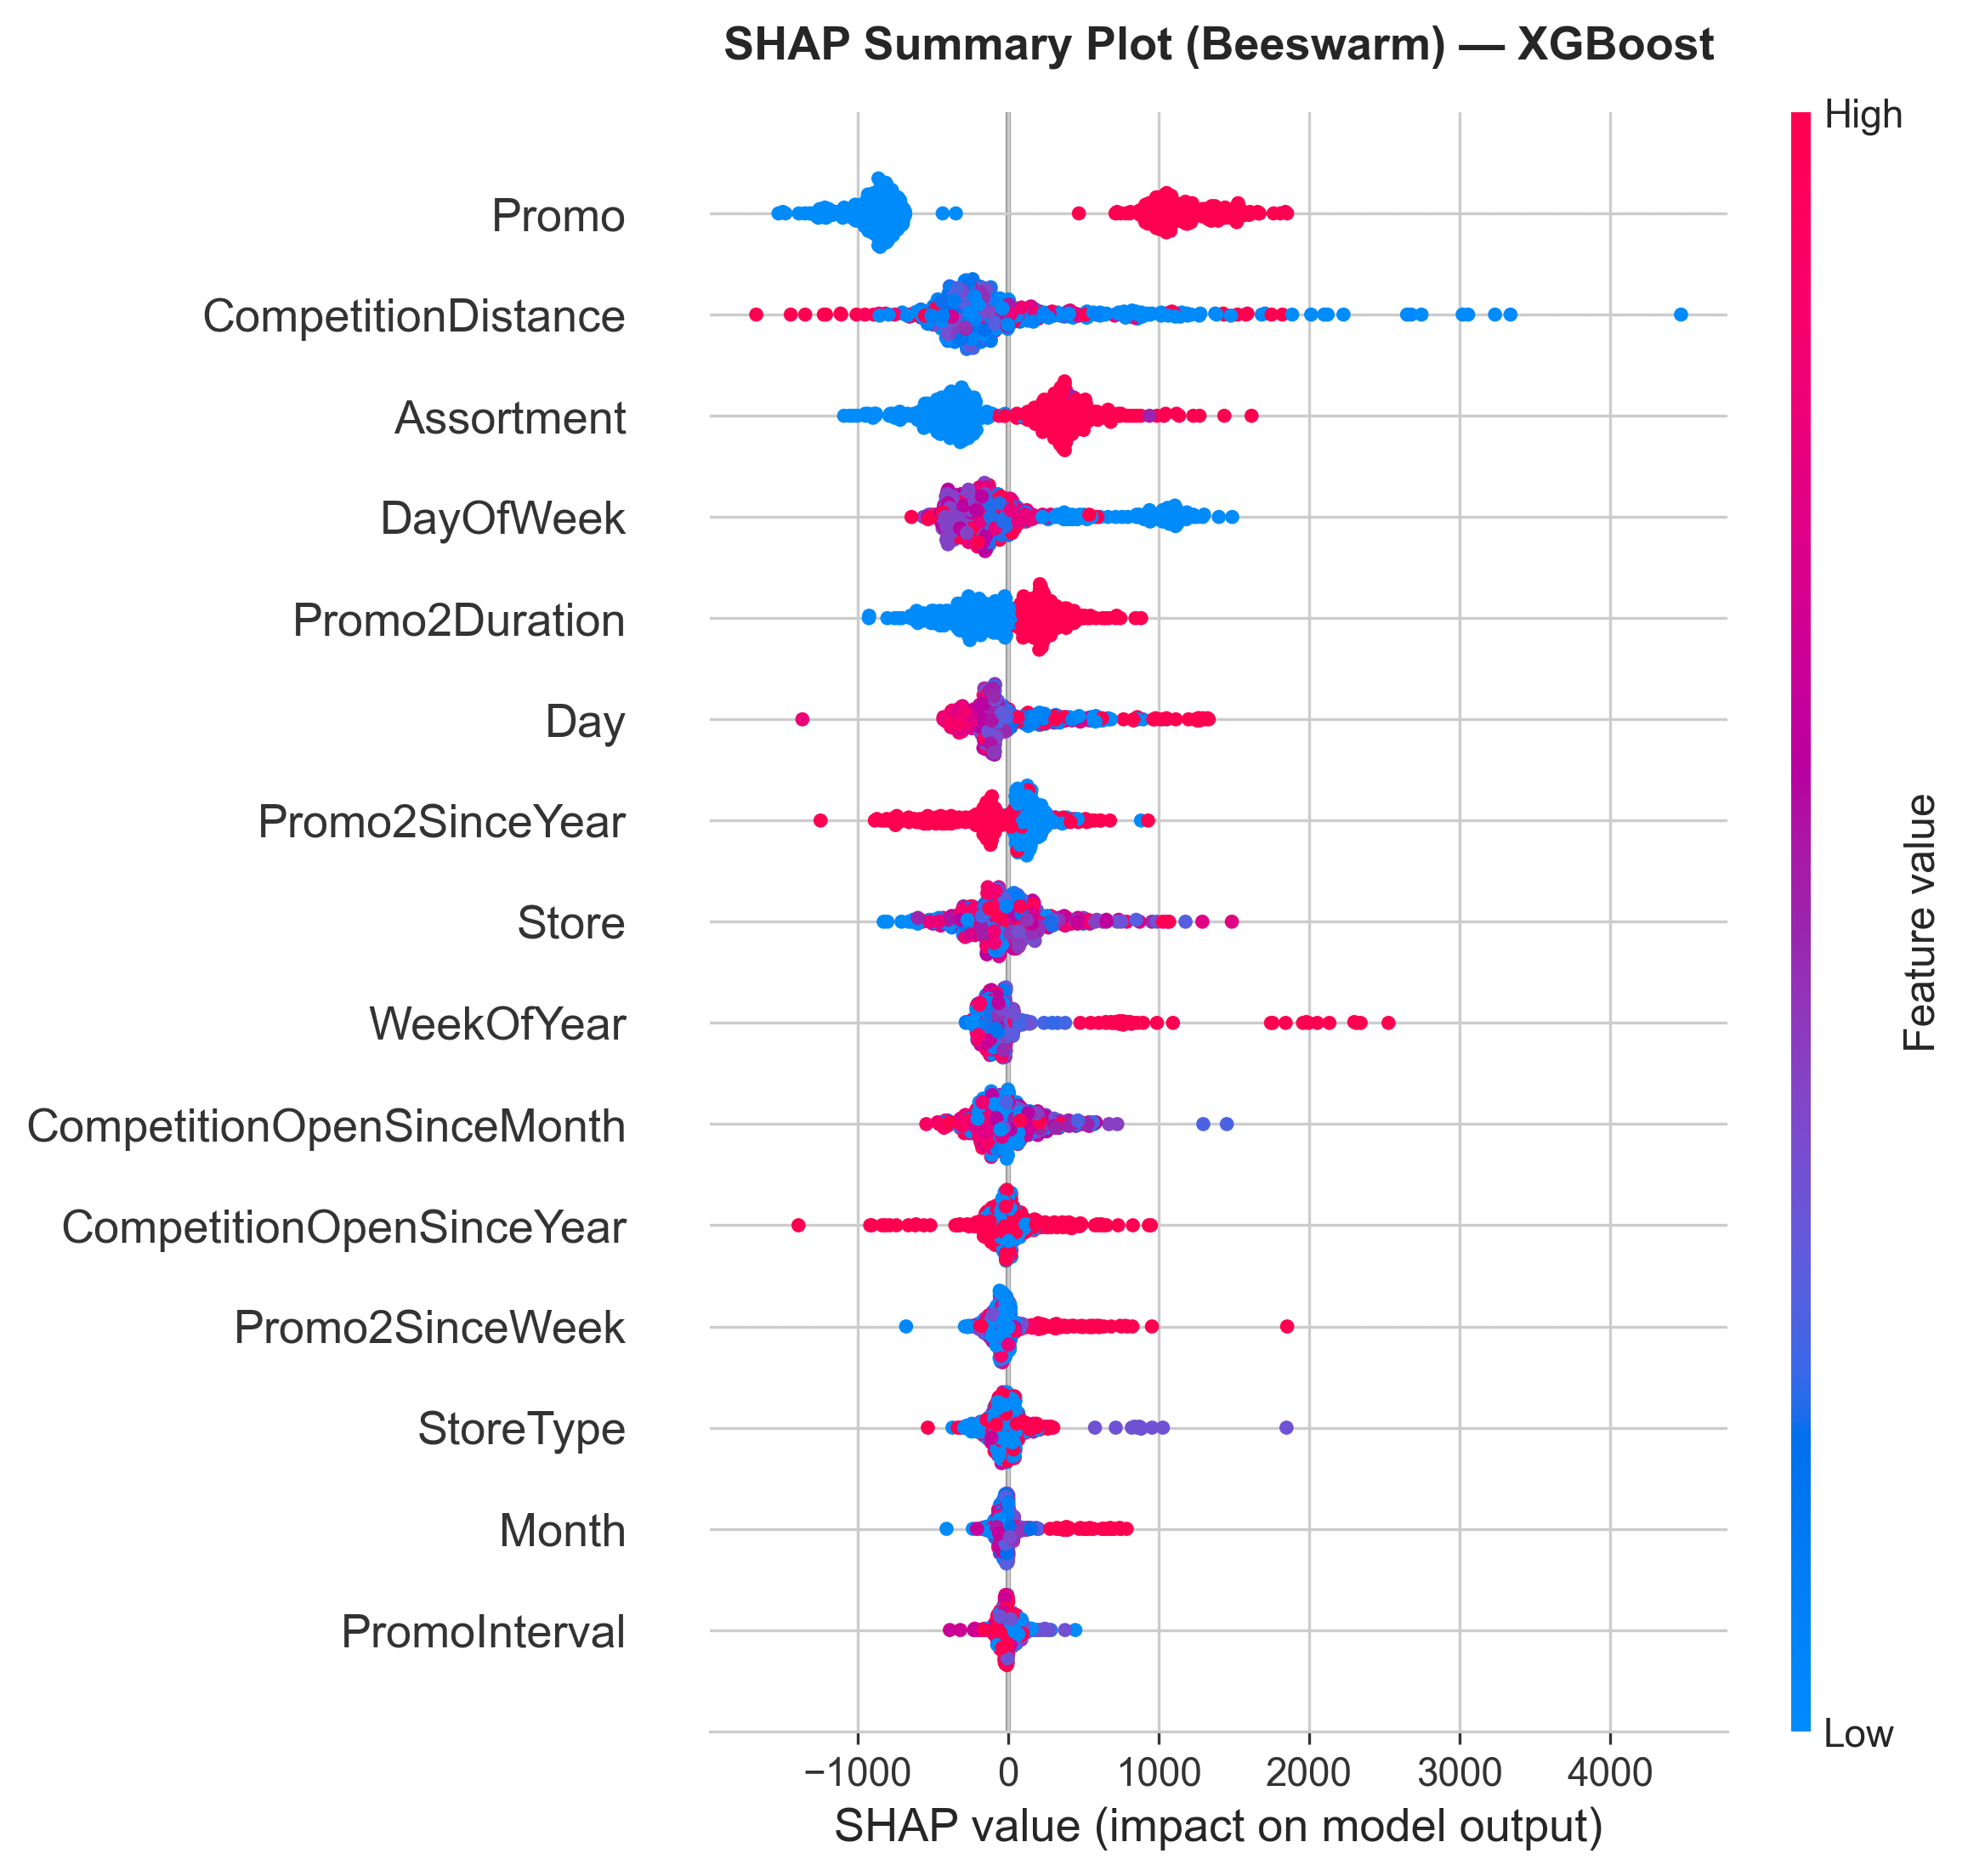
\includegraphics[width=\columnwidth]{shap_summary_xgb.png}
    \caption{SHAP beeswarm summary plot (XGBoost, $n=600$). Colour encodes feature value; horizontal position shows contribution direction and magnitude.}
    \label{fig:beeswarm}
\end{figure}

\texttt{CompetitionDistance} is the highest-ranked feature (0.193). Fig.~\ref{fig:dependence} reveals a counterintuitive pattern: stores within 500~m of a competitor receive a mean SHAP of $+$\euro974, whereas stores beyond 15~km average $-$\euro114. Rather than penalising proximity, the model has learned that short competition distance proxies for dense commercial zones with high customer footfall — a confound that dominates the direct competitive effect in the Rossmann network. Effects are highly non-linear and flatten beyond $\sim$5~km; the interaction with assortment type (colour) explains additional variance.

\begin{figure}[t]
    \centering
    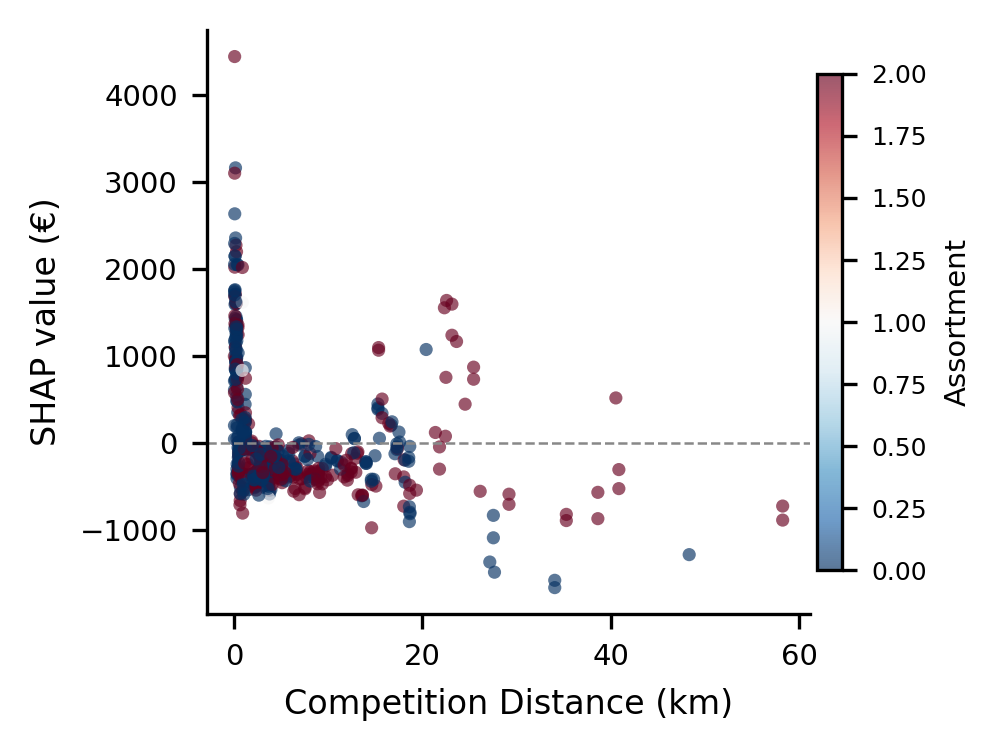
\includegraphics[width=\columnwidth]{shap_dependence_cd.png}
    \caption{SHAP dependence plot for \texttt{CompetitionDistance} (XGBoost, $n=600$), coloured by assortment type. Mean SHAP is $+$\euro974 for distances below 500~m and $-$\euro114 beyond 15~km, with a steep non-linear transition.}
    \label{fig:dependence}
\end{figure}

\texttt{Promo} (0.182) is the most directly controllable driver: active promotional days average a mean SHAP of $+$\euro1{,}189, versus $-$\euro907 on non-promotional days. Store identity (0.167) captures persistent local effects — demographics, foot traffic, customer loyalty — indicating that chain-level aggregate predictions systematically underperform store-specific models. \texttt{DayOfWeek} (0.066) reflects the weekly sales cycle, with weekend attributions leading weekdays in the beeswarm plot.

\subsection{Store-Level Prediction Explanation}

Fig.~\ref{fig:waterfall} shows the SHAP waterfall plot for Store~161, a validation sample from Week~16 of 2013 (mid-April, Day~15) with \emph{no} active standard promotion (\texttt{Promo}~=~0). Starting from the dataset mean $E[f(X)]$~=~\euro6,955, the absence of a promotion is by far the dominant factor: the model assigns $-$\euro1,248 to this store-day — more negative than the global Promo\,=\,0 mean of $-$\euro907, indicating this store is especially promotion-sensitive. A Monday (\texttt{DayOfWeek}~=~1) adds $+$\euro467, but not being at the start of the month subtracts $-$\euro467. The competitor at 2,970~m reduces the prediction by $-$\euro392, while the store's assortment type recovers $+$\euro332. The sum of all contributions yields a final prediction of $f(x)$~=~\euro5,551.

\begin{figure}[t]
    \centering
    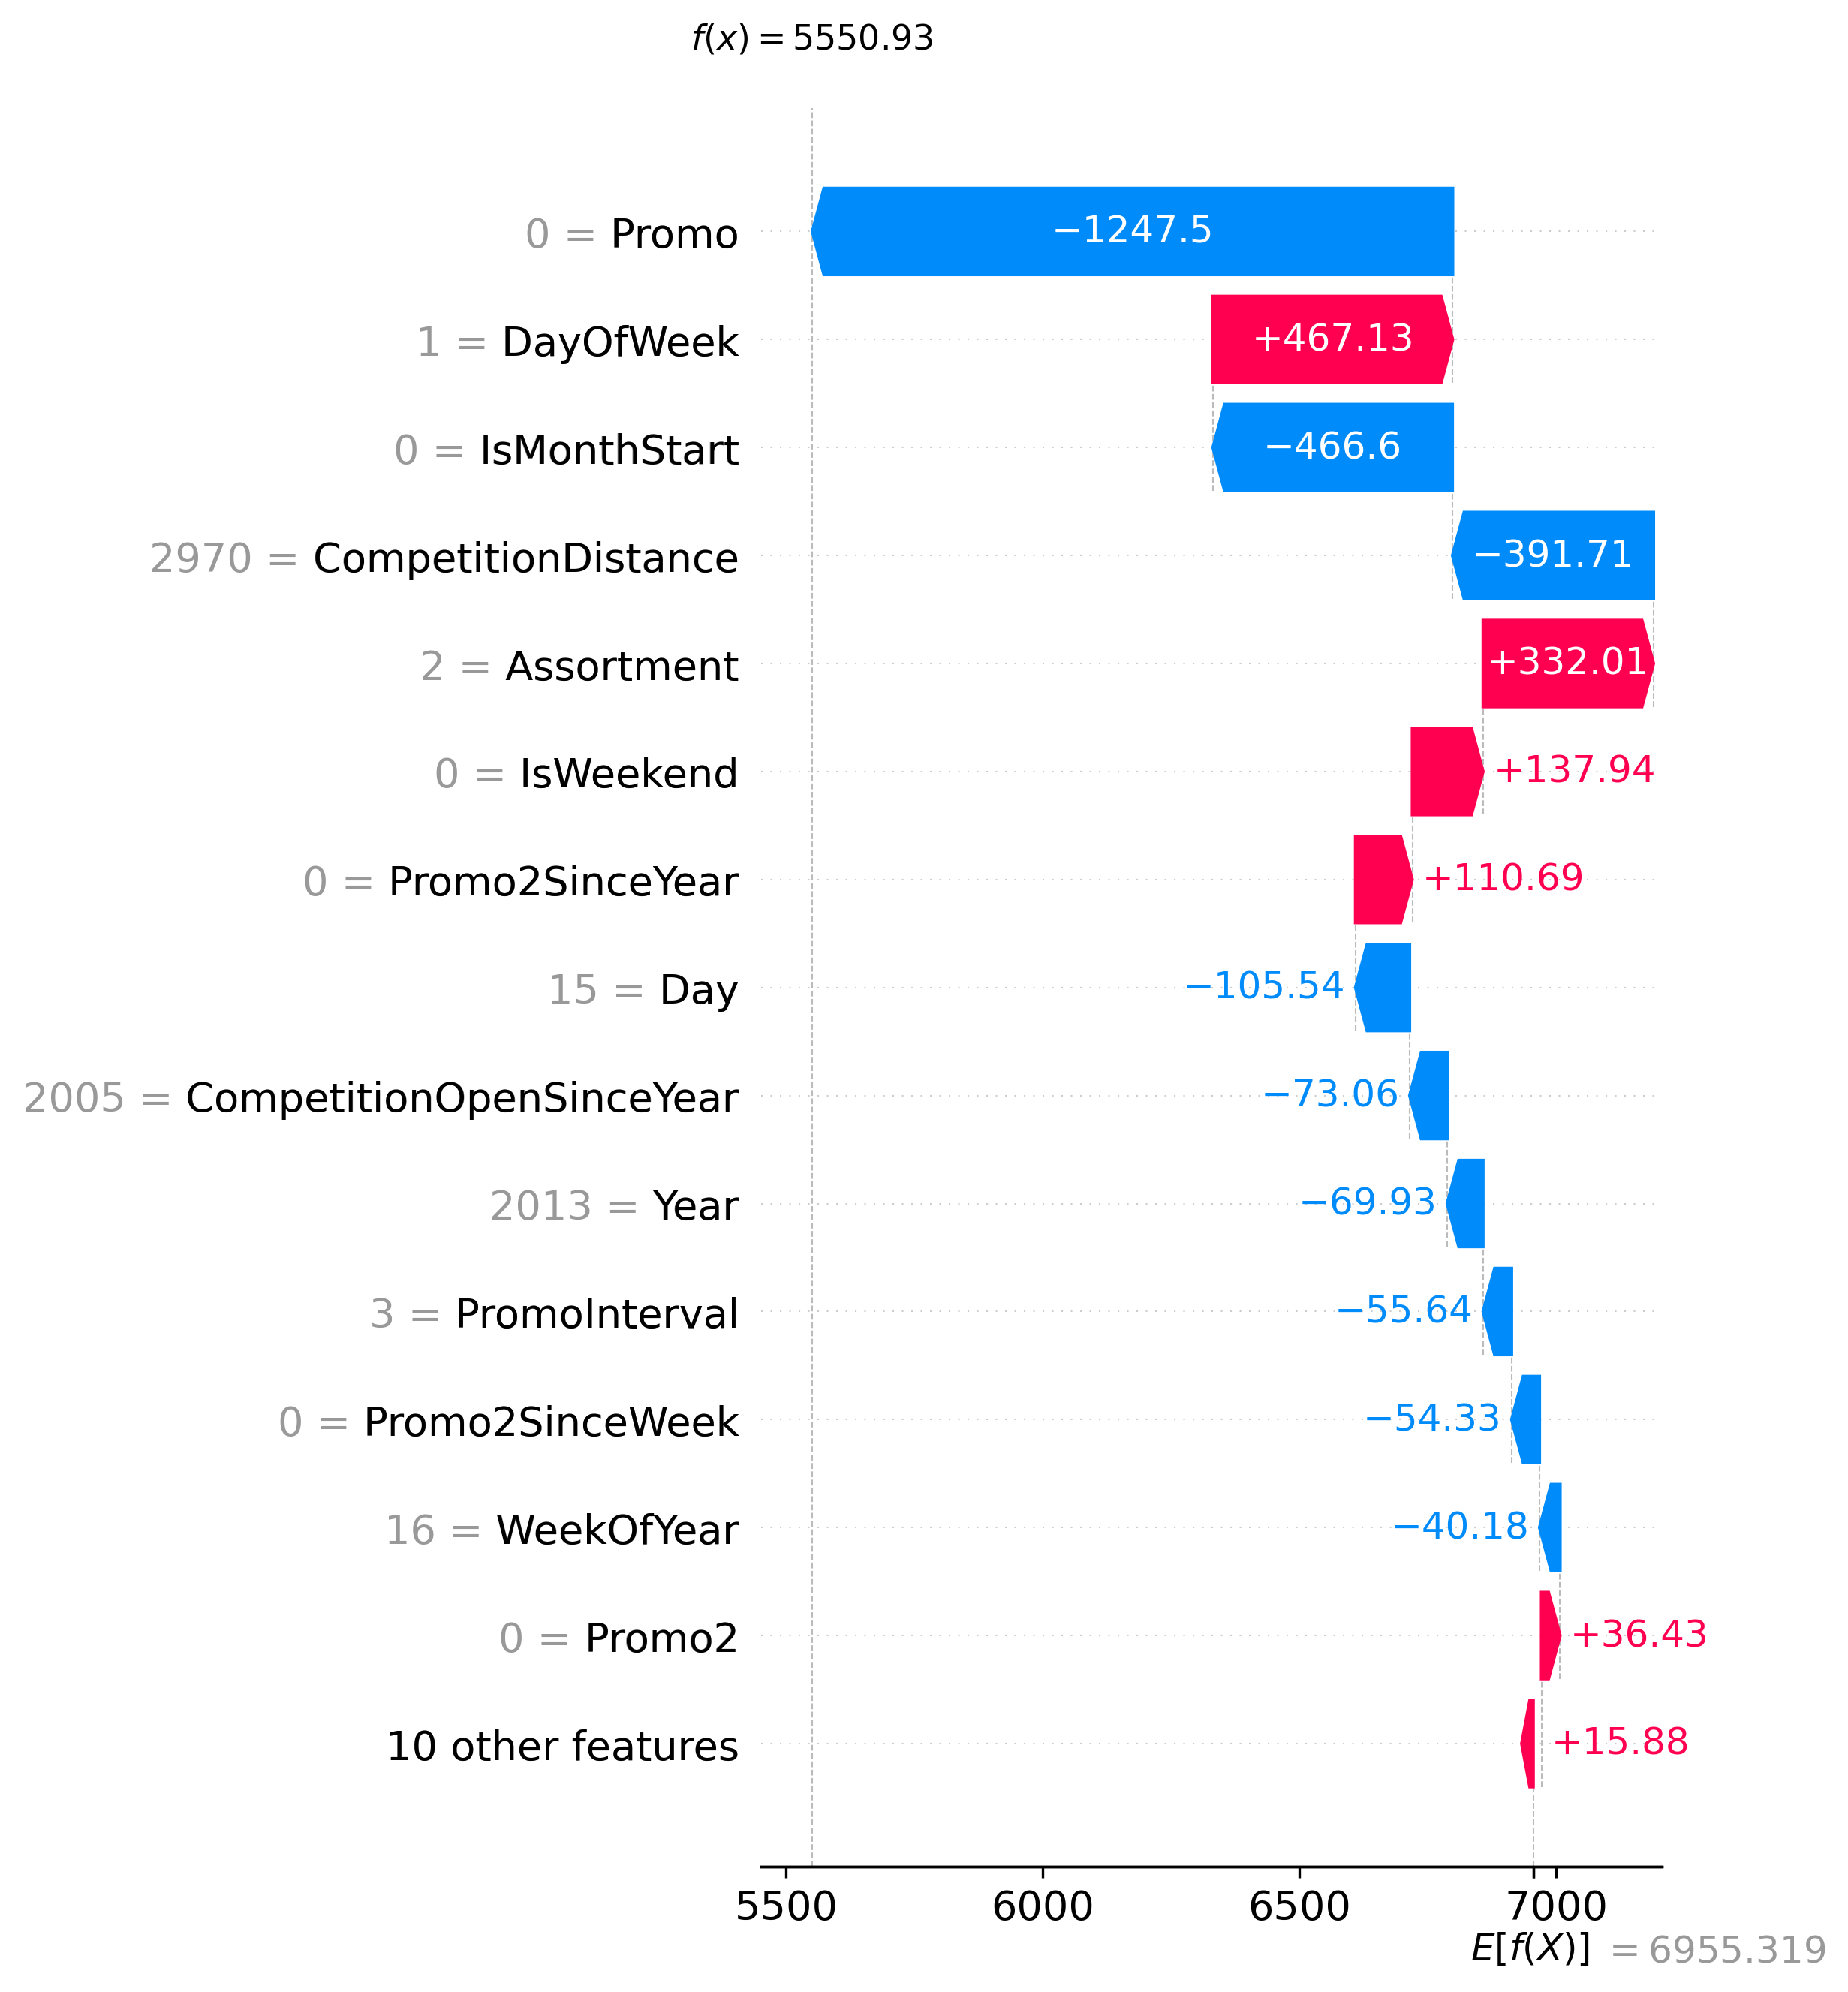
\includegraphics[width=\columnwidth]{shap_waterfall.png}
    \caption{SHAP waterfall plot — Store~161, Week~16 of 2013 (no active promotion, Day~15). All contributions in EUR. Baseline $E[f(X)]$~=~\euro6,955; prediction $f(x)$~=~\euro5,551. The absent promotion is the dominant driver ($-$\euro1,248).}
    \label{fig:waterfall}
\end{figure}

This decomposition is directly actionable: activating a standard promotion would be expected to shift the prediction by approximately $+$\euro1,248 for this specific store-day. The assortment and competitor effects are structural; the promotional decision is the immediate operational lever. All values are read from the model output, not from population averages.

% -------------------------------------------------------
\section{Conclusion}
\label{sec:conclusion}
% -------------------------------------------------------

This study benchmarked Linear Regression, Random Forest, and XGBoost on the Rossmann dataset and applied TreeSHAP to produce auditable, store-level predictions. XGBoost achieved the strongest in-sample generalisation ($R^{2}$~=~0.8512, MAPE~=~13.78\%), and SHAP analysis revealed that competition proximity, promotional activity, and store identity are the primary drivers of daily sales variance. Notably, \texttt{CompetitionDistance} showed a positive SHAP effect at short distances, reflecting commercial-zone density rather than a direct competitive penalty — a finding not recoverable from feature importance alone. The waterfall explanation for Store~161 demonstrated that individual predictions can be decomposed into EUR-valued contributions that are directly actionable by a store manager. The study is an interpolation experiment on 2013--2015 data and does not validate true out-of-sample forecasting.

Two limitations are most consequential. First, the random 80/20 split measures generalisation within the observed time window; a temporal split (train 2013--2014, test 2015) with a separate held-out test set would give an honest forecasting evaluation. Second, unobserved external factors — weather, local events, macroeconomic conditions — contribute to residual error on extreme-sales days. Third, reported metrics are point estimates from a single random seed; variance across splits was not estimated. Future work should evaluate LightGBM~\cite{ke2017} and CatBoost~\cite{prokhorenkova2018}, incorporate external data sources, and validate on broader benchmarks such as the M5 or Walmart Sales datasets.

\subsection*{AI Disclosure}
Portions of this manuscript and supporting analysis code were drafted or refined with assistance from Claude (Anthropic). All experimental design, model training, and result verification were performed by the author, who reviewed and validated the final text and code.

\balance
\begin{thebibliography}{14}

\bibitem{hyndman2021}
R.~J. Hyndman and G.~Athanasopoulos,
\emph{Forecasting: Principles and Practice}, 3rd~ed. OTexts, 2021.

\bibitem{box1994}
G.~E.~P. Box and G.~M. Jenkins,
\emph{Time Series Analysis: Forecasting and Control}, 3rd~ed. Prentice Hall, 1994.

\bibitem{grinsztajn2022}
L.~Grinsztajn, E.~Oyallon, and G.~Varoquaux,
``Why tree-based models still outperform deep learning on tabular data,''
in \emph{Adv. Neural Inf. Process. Syst.}, vol.~35, 2022.

\bibitem{lundberg2017}
S.~M. Lundberg and S.-I. Lee,
``A unified approach to interpreting model predictions,''
in \emph{Adv. Neural Inf. Process. Syst.}, vol.~30, 2017, pp.~4765--4774.

\bibitem{chen2016}
T.~Chen and C.~Guestrin,
``XGBoost: A scalable tree boosting system,''
in \emph{Proc. 22nd ACM SIGKDD}, 2016, pp.~785--794.

\bibitem{ke2017}
G.~Ke et al.,
``LightGBM: A highly efficient gradient boosting decision tree,''
in \emph{Adv. Neural Inf. Process. Syst.}, vol.~30, 2017.

\bibitem{prokhorenkova2018}
L.~Prokhorenkova et al.,
``CatBoost: Unbiased boosting with categorical features,''
in \emph{Adv. Neural Inf. Process. Syst.}, vol.~31, 2018.

\bibitem{hochreiter1997}
S.~Hochreiter and J.~Schmidhuber,
``Long short-term memory,''
\emph{Neural Computation}, vol.~9, no.~8, pp.~1735--1780, 1997.

\bibitem{lim2021}
B.~Lim et al.,
``Temporal fusion transformers for interpretable multi-horizon time series forecasting,''
\emph{Int. J. Forecasting}, vol.~37, no.~4, pp.~1748--1764, 2021.

\bibitem{shwartz2022}
R.~Shwartz-Ziv and A.~Armon,
``Tabular data: Deep learning is not all you need,''
\emph{Inf. Fusion}, vol.~81, pp.~84--90, 2022.

\bibitem{lundberg2020}
S.~M. Lundberg et al.,
``From local explanations to global understanding with explainable AI for trees,''
\emph{Nature Mach. Intell.}, vol.~2, pp.~56--67, 2020.

\bibitem{ribeiro2016}
M.~T. Ribeiro, S.~Singh, and C.~Guestrin,
```Why should I trust you?': Explaining the predictions of any classifier,''
in \emph{Proc. 22nd ACM SIGKDD}, 2016, pp.~1135--1144.

\bibitem{dzyabura2019}
D.~Dzyabura and J.~R. Hauser,
``Recommending products when consumers learn their preference weights,''
\emph{Marketing Sci.}, vol.~38, no.~3, pp.~417--441, 2019.

\bibitem{breiman2001}
L.~Breiman,
``Random forests,''
\emph{Mach. Learn.}, vol.~45, pp.~5--32, 2001.

\end{thebibliography}

\end{document}
